% Copyright 2004 by Till Tantau <tantau@users.sourceforge.net>.
%
% In principle, this file can be redistributed and/or modified under
% the terms of the GNU Public License, version 2.
%
% However, this file is supposed to be a template to be modified
% for your own needs. For this reason, if you use this file as a
% template and not specifically distribute it as part of a another
% package/program, I grant the extra permission to freely copy and
% modify this file as you see fit and even to delete this copyright
% notice. 

\documentclass{beamer}

\usepackage{blindtext}
\usepackage{tcolorbox}
\usepackage{soul}

\usefonttheme{professionalfonts} % using non standard fonts for beamer
\usefonttheme{serif} % default family is serif
%\usepackage{fontspec}
%\setmainfont{Liberation Serif}

% There are many different themes available for Beamer. A comprehensive
% list with examples is given here:
% http://deic.uab.es/~iblanes/beamer_gallery/index_by_theme.html
% You can uncomment the themes below if you would like to use a different
% one:
%\usetheme{AnnArbor}
%\usetheme{Antibes}
%\usetheme{Bergen}
%\usetheme{Berkeley}
%\usetheme{Berlin}
%\usetheme{Boadilla}
%\usetheme{boxes}
%\usetheme{CambridgeUS}
%\usetheme{Copenhagen}
%\usetheme{Darmstadt}
\usetheme{default}
%\usetheme{Frankfurt}
%\usetheme{Goettingen}
%\usetheme{Hannover}
%\usetheme{Ilmenau}
%\usetheme{JuanLesPins}
%\usetheme{Luebeck}
%\usetheme{Madrid}
%\usetheme{Malmoe}
%\usetheme{Marburg}
%\usetheme{Montpellier}
%\usetheme{PaloAlto}
%\usetheme{Pittsburgh}
%\usetheme{Rochester}
%\usetheme{Singapore}
%\usetheme{Szeged}
%\usetheme{Warsaw}



\title{Introduction to Signal Processing}

% A subtitle is optional and this may be deleted
\subtitle{Lecture 4: \textbf{Continuous-time Linear Time Invariant Systems}}

\author{Sivakumar Balasubramanian}
% - Give the names in the same order as the appear in the paper.
% - Use the \inst{?} command only if the authors have different
%   affiliation.

\institute[Christian Medical College] % (optional, but mostly needed)
{
  \inst{}%
  Department of Bioengineering\\
  Christian Medical College, Bagayam\\
  Vellore 632002
}
% - Use the \inst command only if there are several affiliations.
% - Keep it simple, no one is interested in your street address.

\date{}
% - Either use conference name or its abbreviation.
% - Not really informative to the audience, more for people (including
%   yourself) who are reading the slides online

\subject{Lecture notes on signal processing}
% This is only inserted into the PDF information catalog. Can be left
% out.

% If you have a file called "university-logo-filename.xxx", where xxx
% is a graphic format that can be processed by latex or pdflatex,
% resp., then you can add a logo as follows:

% \pgfdeclareimage[height=0.5cm]{university-logo}{university-logo-filename}
% \logo{\pgfuseimage{university-logo}}

% Delete this, if you do not want the table of contents to pop up at
% the beginning of each subsection:
\AtBeginSubsection[]
{
  \begin{frame}<beamer>{Outline}
    \tableofcontents[currentsection,currentsubsection]
  \end{frame}
}

% Let's get started
\begin{document}

\begin{frame}
  \titlepage
\end{frame}

% OPERATIONS ON SIGNALS
\begin{frame}{Operations on signals}

\begin{columns}
	\begin{column}{.6\linewidth}
	\textbf{Operations on the dependent variable}
	\begin{itemize}
		\item \textbf{Scaling}: $y(t) = ax(t)$
		\item \textbf{Addition}: $y(t) = x_1(t) + x_2(t)$
		\item \textbf{Differentiation}: $y(t) = \frac{d}{dt}x(t)$
		\item \textbf{Integration}: $y(t) = \int_{-\infty}^{t}x(t)dt$
	\end{itemize}
	\end{column}

	\begin{column}{.5\linewidth}
	\textbf{Operations on the independent variable}
	\begin{itemize}
		\item \textbf{Time shifting}: $y(t) = x(t - \tau), \tau \in \mathbb{R}$
		\item \textbf{Time Scaling}: $y(t) = x(at)$
	\end{itemize}
	\end{column}
\end{columns}

\end{frame}

% TIME SHIFTING
\begin{frame}{Operation on the independent variable: \textbf{Time shifting}}

Consider $x(t)$ shown below,

\begin{figure}
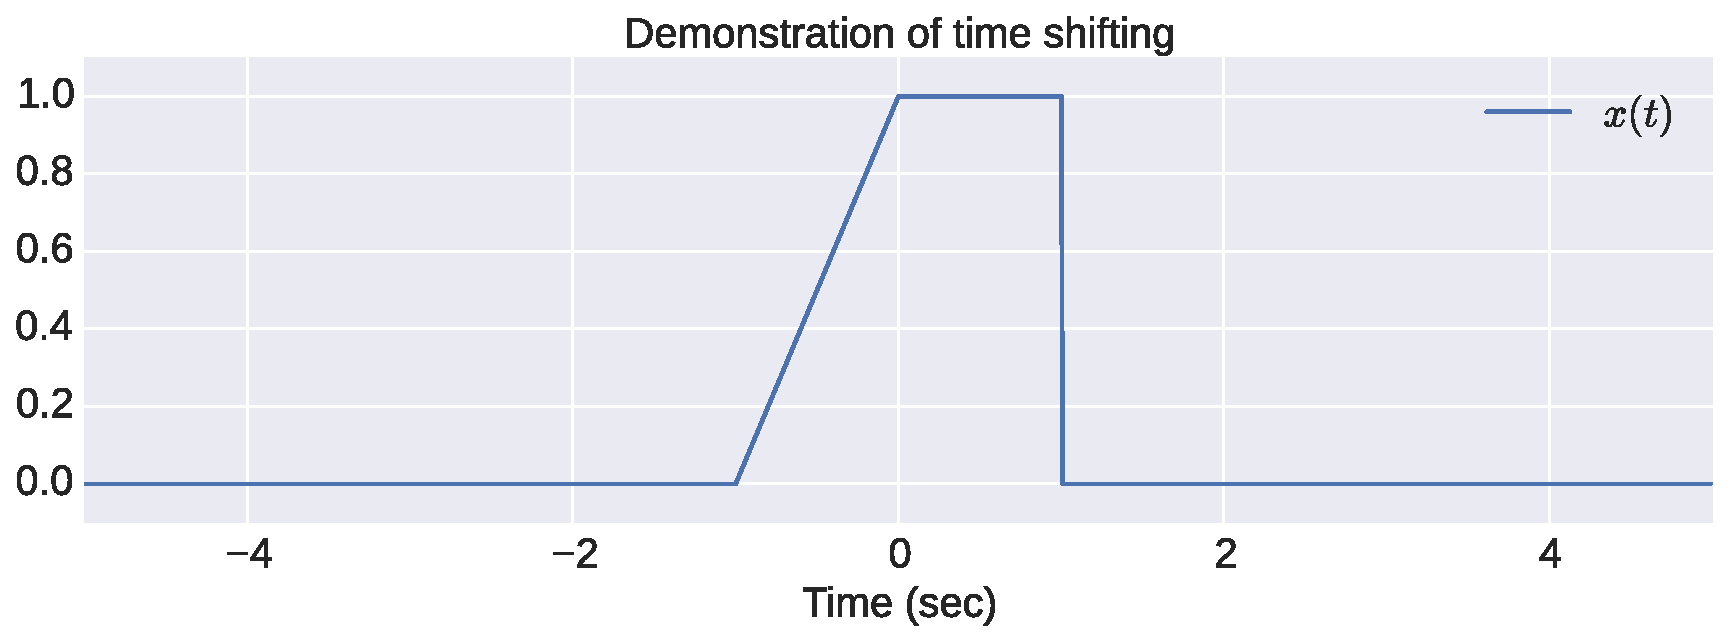
\includegraphics[width=\textwidth]{img/tshift0.eps}
\end{figure}

What does $x(t-1.5)$ look like?

\end{frame}

% TIME SHIFTING
\begin{frame}{Operation on the independent variable: \textbf{Time shifting}}

\begin{figure}
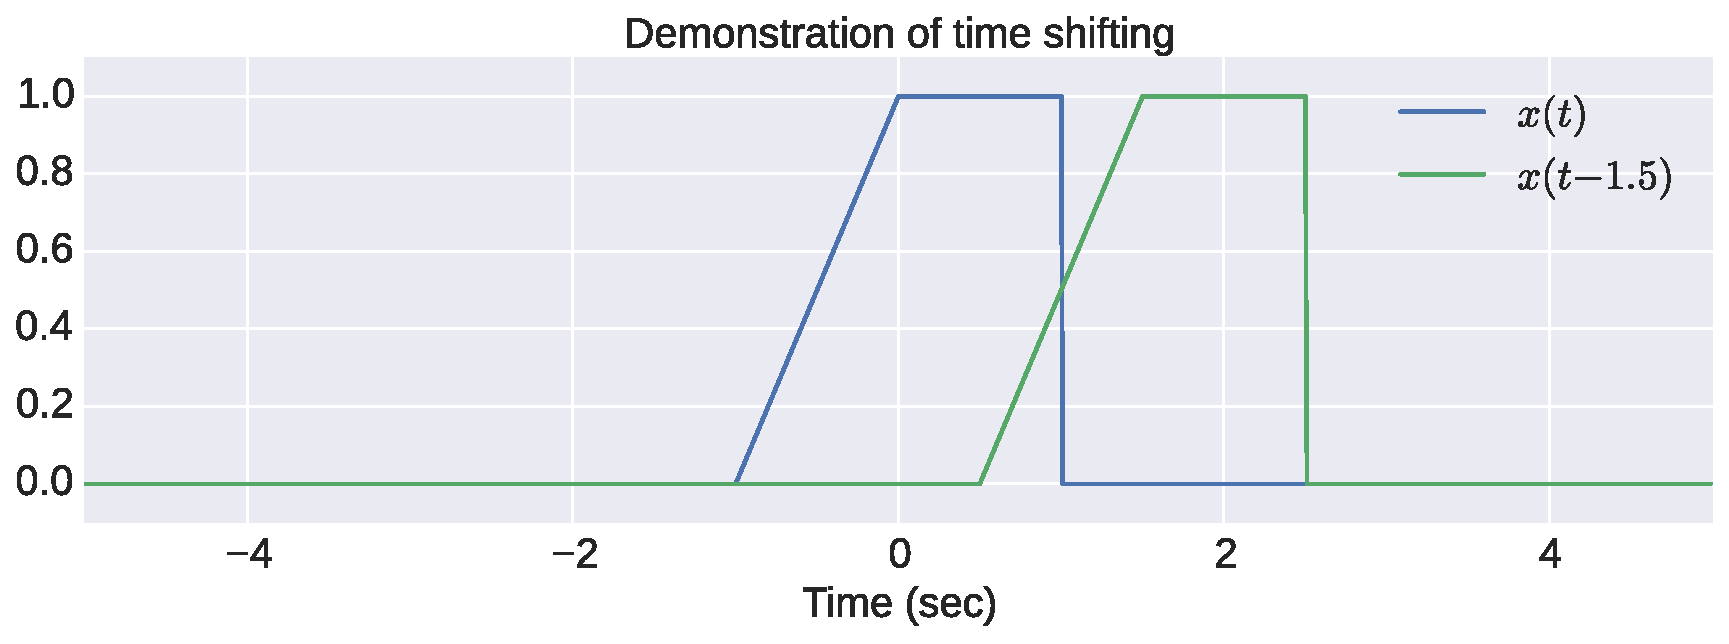
\includegraphics[width=\textwidth]{img/tshift1.eps}
\end{figure}

What does $x(t+2.5)$ look like?

\end{frame}

% TIME SHIFTING
\begin{frame}{Operation on the independent variable: \textbf{Time shifting}}

\begin{figure}
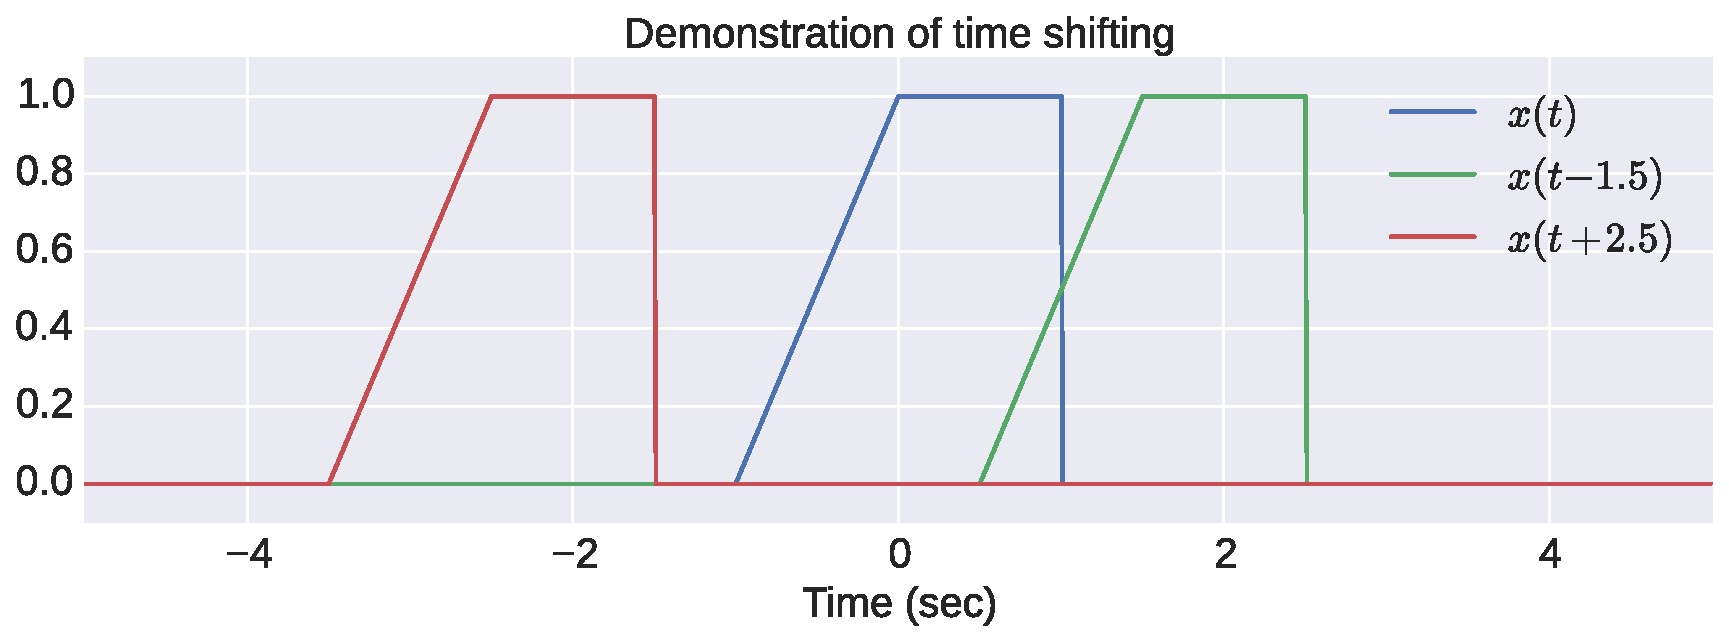
\includegraphics[width=\textwidth]{img/tshift2.eps}
\end{figure}

Effect of $\tau$ on time shifting operation,
\[
x(t-\tau) \longrightarrow \begin{cases}
\tau > 0 & \text{Delays signal} \\
\tau < 0 & \text{Forwards signal} \\
\end{cases}
\]
\end{frame}

% TIME SCALING
\begin{frame}{Operation on the independent variable: \textbf{Time scaling}}

\begin{figure}
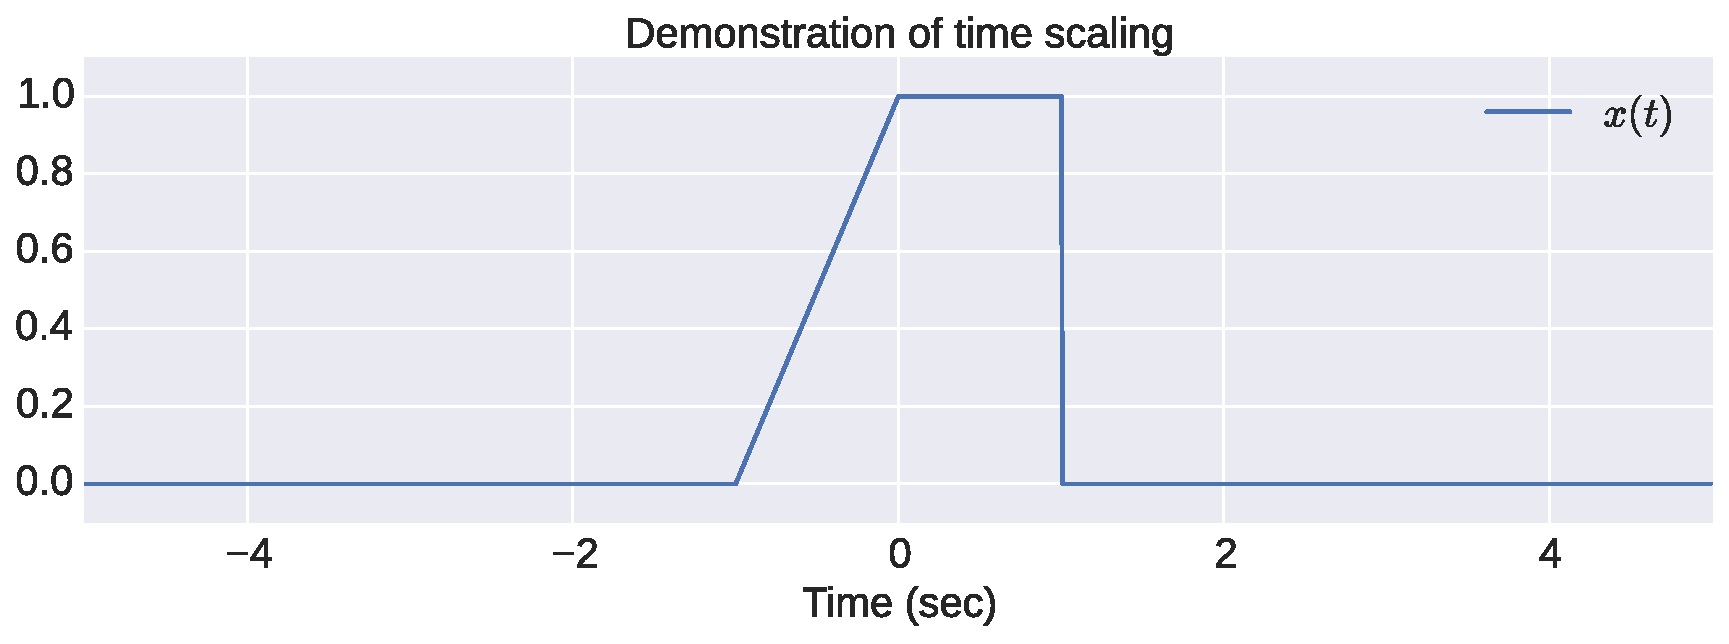
\includegraphics[width=\textwidth]{img/tscale0.eps}
\end{figure}

What does $x(0.5t)$ look like?

\end{frame}

% TIME SCALING
\begin{frame}{Operation on the independent variable: \textbf{Time scaling}}

\begin{figure}
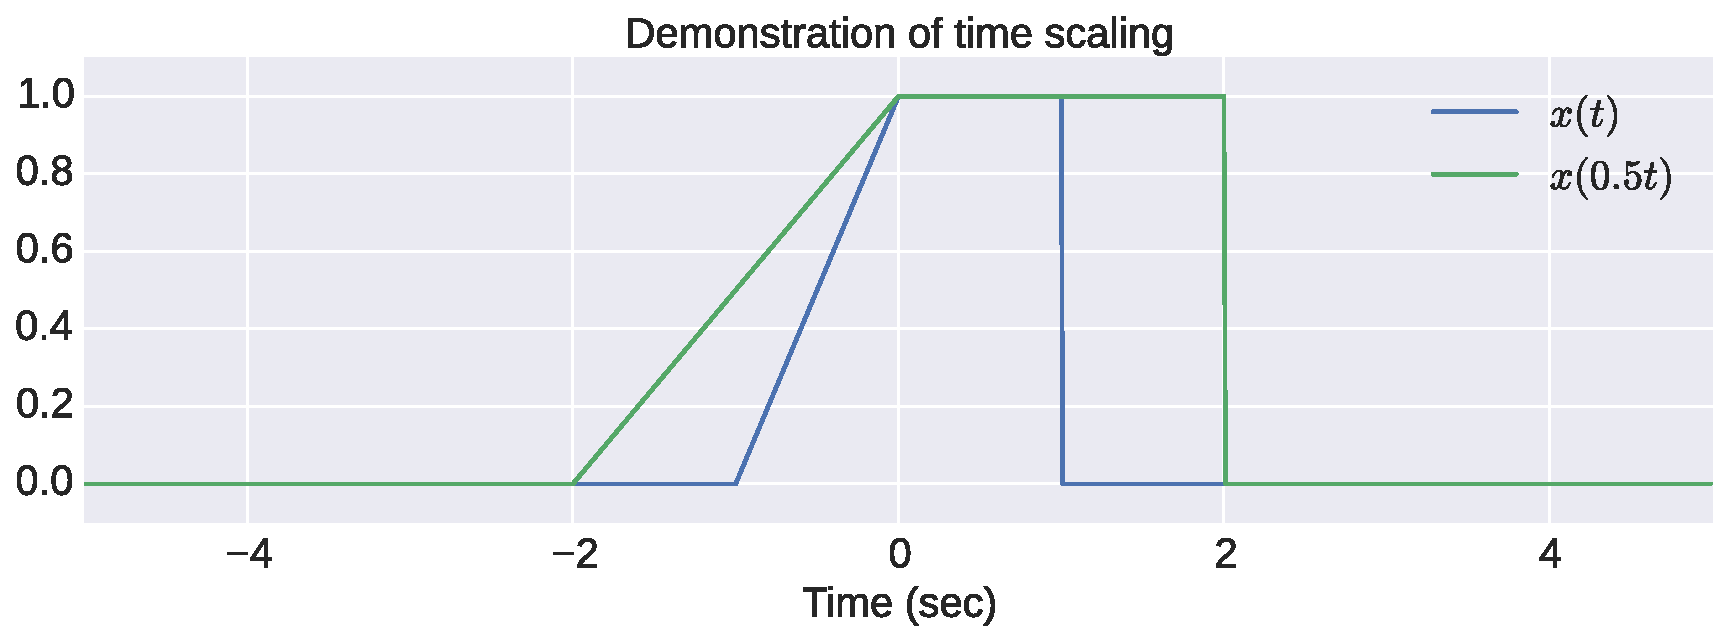
\includegraphics[width=\textwidth]{img/tscale1.eps}
\end{figure}

What does $x(2.5t)$ look like?

\end{frame}

% TIME SCALING
\begin{frame}{Operation on the independent variable: \textbf{Time scaling}}

\begin{figure}
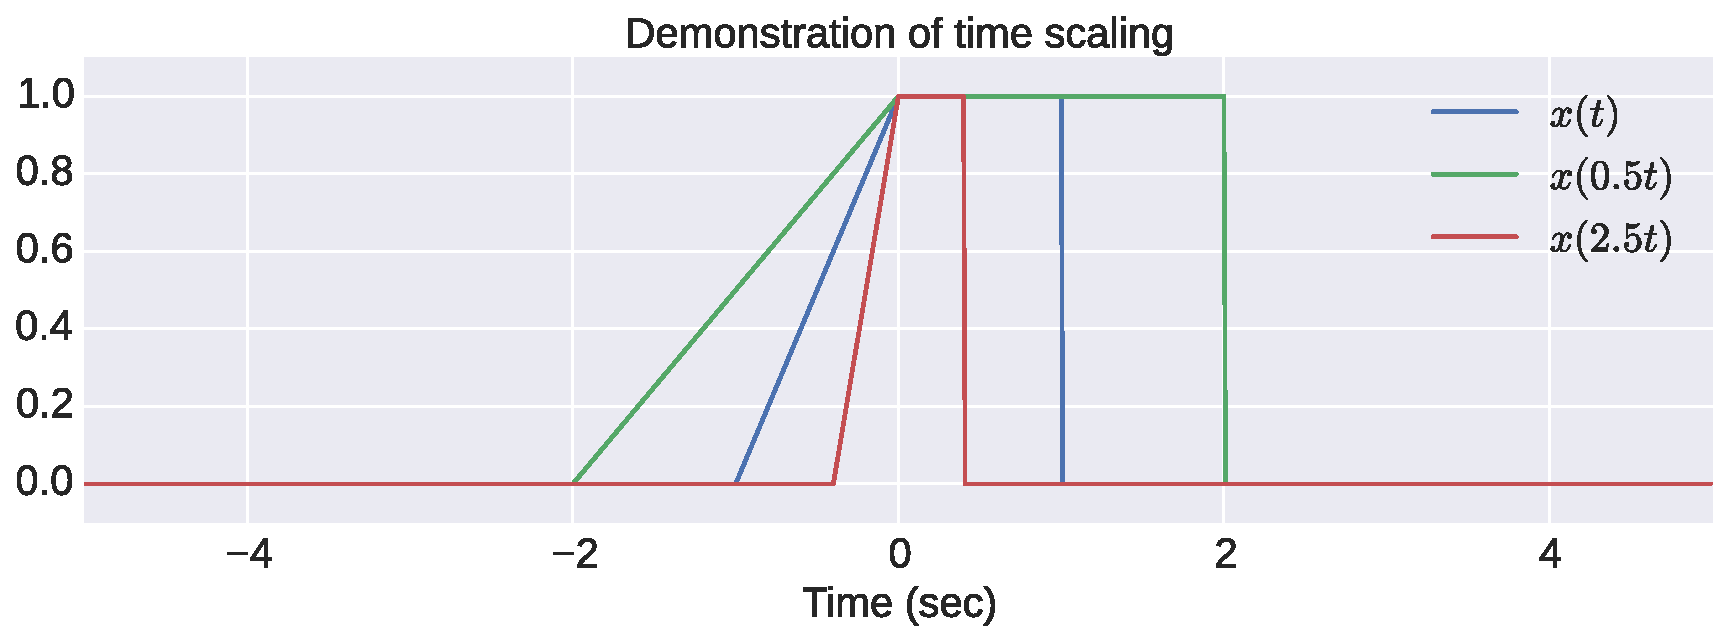
\includegraphics[width=\textwidth]{img/tscale2.eps}
\end{figure}

What does $x(-1.5t)$ look like?

\end{frame}

% TIME SCALING
\begin{frame}{Operation on the independent variable: \textbf{Time scaling}}

\begin{figure}
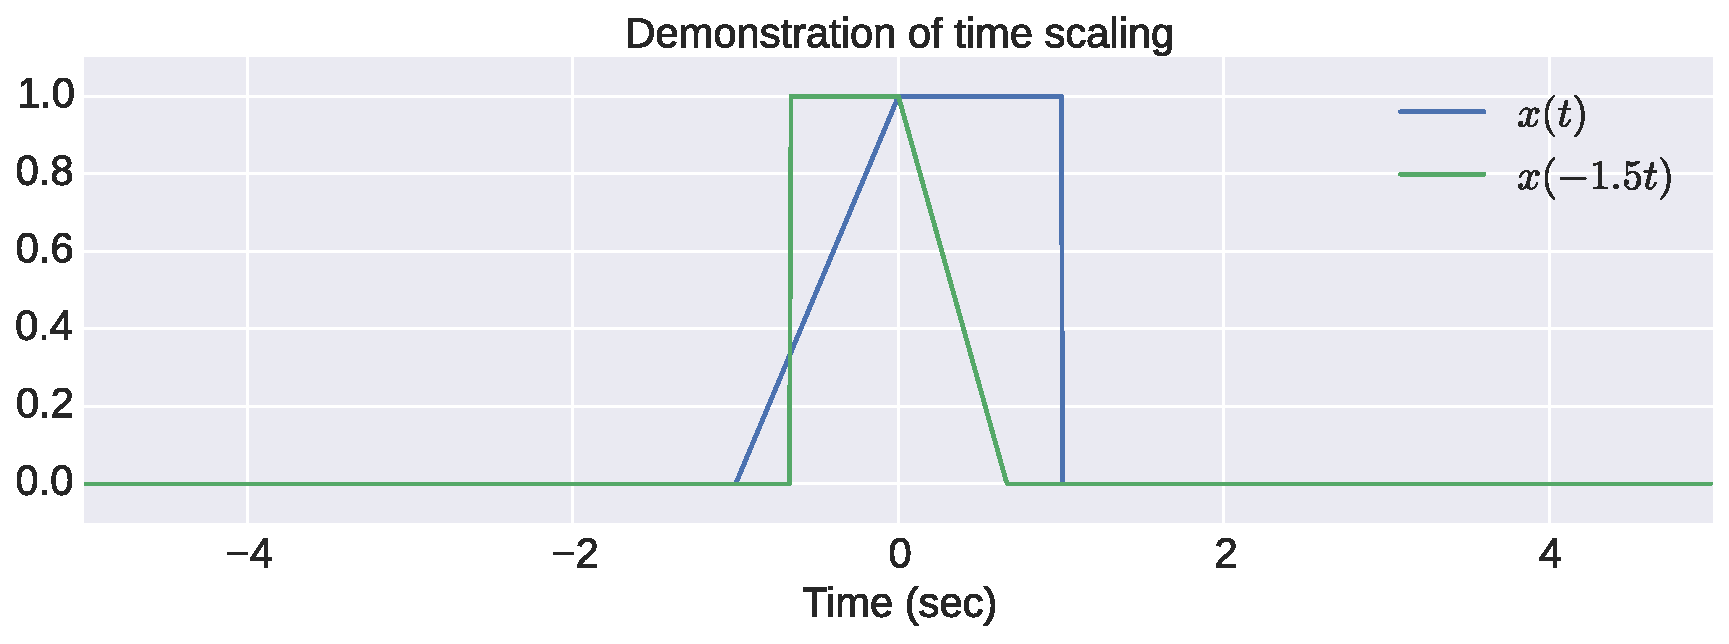
\includegraphics[width=\textwidth]{img/tscale3.eps}
\end{figure}

Effect of $a$ on time scaling operation,
\[
x(at) \longrightarrow \begin{cases}
0 < a < 1 & \text{Exapands signal} \\
1 < a < \infty & \text{Shrinks signal} \\
-1 < a < 0 & \text{Inverts and expands signal} \\
-\infty < a < -1 & \text{Inverts and shrinks signal} \\
\end{cases}
\]
\end{frame}

% LINEAR TIME-INVARIANT SYSTEMS
\begin{frame}{Continous-time LTI Systems}

Remember the definitions of \textbf{linearity} and \textbf{time invariance}?

\[ x_i(t) \mapsto y_i(t) \implies \sum a_ix_i(t - \tau_i) \mapsto a_i \sum y_i(t - \tau_i) \]

\vspace{10mm}

\textbf{Why are we interested in LTI systems?}
\begin{itemize}
\item A reasonable approximation of real world systems.
\item Well developed theory and tools for analysis and synthesis
\end{itemize}

\end{frame}

% LINEAR TIME-INVARIANT SYSTEMS
\begin{frame}{Characterization of continous-time LTI Systems}

\begin{itemize}
\item The analysis and synthesis of continuous time LTI system can be done either in the \textbf{time domain} or the \textbf{frequency domain}.
\item Four ways to look at the time domain characteristics:
\begin{itemize}
\item Impulse response
\item Differential equations
\item State space representation
\item Block diagram representation
\end{itemize}
\end{itemize}

\end{frame}

% IMPULSE RESPONSE
\begin{frame}{Impulse Response of a LTI system}

\begin{itemize}
\item We know everything about a system $H$, if we the output of the system $y(t)$ for any arbitrary input $x(t)$.
\item A brute force method is to do so will be to tabulate all possible inputs and outputs!
\item \ul{LTI systems allow a much more abbreviated representation}.
\item Let us assume that we have a set of inputs $x_i(t)$ with known outputs for a given LTI system $H$, such that
\[ H\{x_i(t)\} = y_i(t)\]
\item This implies that if there is an input $x(t)$ that is a linear combination of time shifted versions on $x_i(t)$, then
\[ H\{x(t)\} = H\left\{ \sum a_ix_i(t-\tau_i) \right\} = \sum a_i H\left\{x_i(t-\tau_i)\right\} \]
\[ H\{x(t)\} = \sum a_iy_i(t)\]
\end{itemize}

\end{frame}

% IMPULSE RESPONSE
\begin{frame}{Impulse Response of a LTI system}

\begin{itemize}
\item Can we choose the signal $x_i(t)$ such that any arbitrary singal $x(t)$ can be represented as a linear combination of time shifted versions of $x_i(t)$?
\pause
\item \textbf{Yes}. The answer is the Dirac delta or impulse function $\delta(t)$.
\pause
\item $\delta(t)$ acts as a value selector. 
\[ \int_{-\infty}^{\infty}f(\tau)\delta(\tau)d\tau = f(0) \]
\pause
\item What do we get here? $\int_{-\infty}^{\infty}f(t-\tau)\delta(\tau)d\tau = ?$
\pause
\[ \int_{-\infty}^{\infty}f(t-\tau)\delta(\tau)d\tau = f(t) \]

\textbf{Note}: $f(\bullet)$ is assumed to be continuous at $t$. 
\end{itemize}

\end{frame}

% IMPULSE RESPONSE
\begin{frame}{Impulse Response of a LTI system}

\begin{itemize}
\item The impulse response $h(t)$ of a system is the output of the system when $\delta(t)$ is applied as an input.
\item We know that, $x(t) = \int_{-\infty}^{\infty} x(\tau) \delta(t - \tau)d\tau$
\[ y(t) = H\{x(t)\} = H\left\{\int_{-\infty}^{\infty}x(\tau)\delta(t - \tau)d\tau \right\} \]
\[ = \int_{-\infty}^{\infty}x(\tau)H\left\{\delta(t - \tau)\right\}d\tau \]
\[= \int_{-\infty}^{\infty}x(\tau)h(t - \tau)d\tau = h(t) * x(t) \]

This is the \textit{convolution integral} .

\end{itemize}

\end{frame}

% IMPULSE RESPONSE
\begin{frame}{Impulse Response of a LTI system}

\begin{itemize}      
\item Properties of the convolution integral
\begin{enumerate}
\item \textit{Commutativity:} 
\[ h(t) * x(t) = x(t) * h(t) \]
\item \textit{Associativity:} 
\[ g(t) * (h(t) * x(t)) = (g(t) * h(t)) * x(t) \]
\item \textit{Connection with the inner product:} 
\[ h(t) * x(t) = \int_{-\infty}^{\infty}x(\tau)h(t - \tau)d\tau = \langle x(t), h^*(t - \tau) \rangle\]
%\textbf{Note:} This is meaningful only when $x(t), h(t) \in \mathcal{L}^2\left(\mathbb{R}\right)$.
\end{enumerate}
\end{itemize}
\end{frame}

% IMPULSE RESPONSE
\begin{frame}{Impulse response of a simple RC circuit}

\begin{figure}
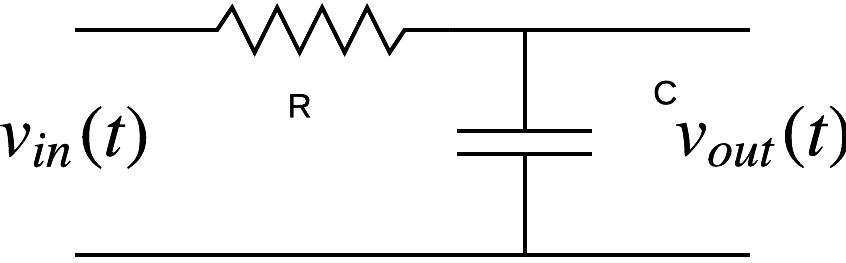
\includegraphics[width=0.5\textwidth]{img/simple_rc.png}
\end{figure}

Here, the output $v_{out}(t)$ is given by,
\[ v_{out}(t) = e^{-t/RC} \left(\frac{1}{RC}\int_{0}^{\infty} {e^{\tau / RC}{v_{in}\left(\tau\right)}}d\tau\right) + v_{out}\left(0\right)e^{-t/RC} \]

Consider the input $x_T(t) = \begin{cases} \frac{1}{T} & 0 \leq t \leq T\\ 0 & \text{Otherwise} \end{cases}$.

\[ \delta(t) = \lim_{T \to 0} x_T(t) \]

Output of the system for $v_{in}(t) = x_T(t)$ will tend toward $h(t)$, when $T \to 0$.

\end{frame}

% IMPULSE RESPONSE
\begin{frame}{Impulse response of a simple RC circuit}

\[ v_{out}(t) = \begin{cases}
0 & t < 0\\
\frac{1}{T}\left(1 - e^{-t/RC}\right) & 0 \leq t \leq T \\
\frac{1}{T}\left(1 - e^{-T/RC}\right)e^{-(t-T)/RC} & t > T \\
\end{cases} \]

Verify that when $T \to 0$, $v_{out}(t) = \frac{1}{RC}e^{-t/RC}, \,\,\, t \geq 0$

\begin{figure}
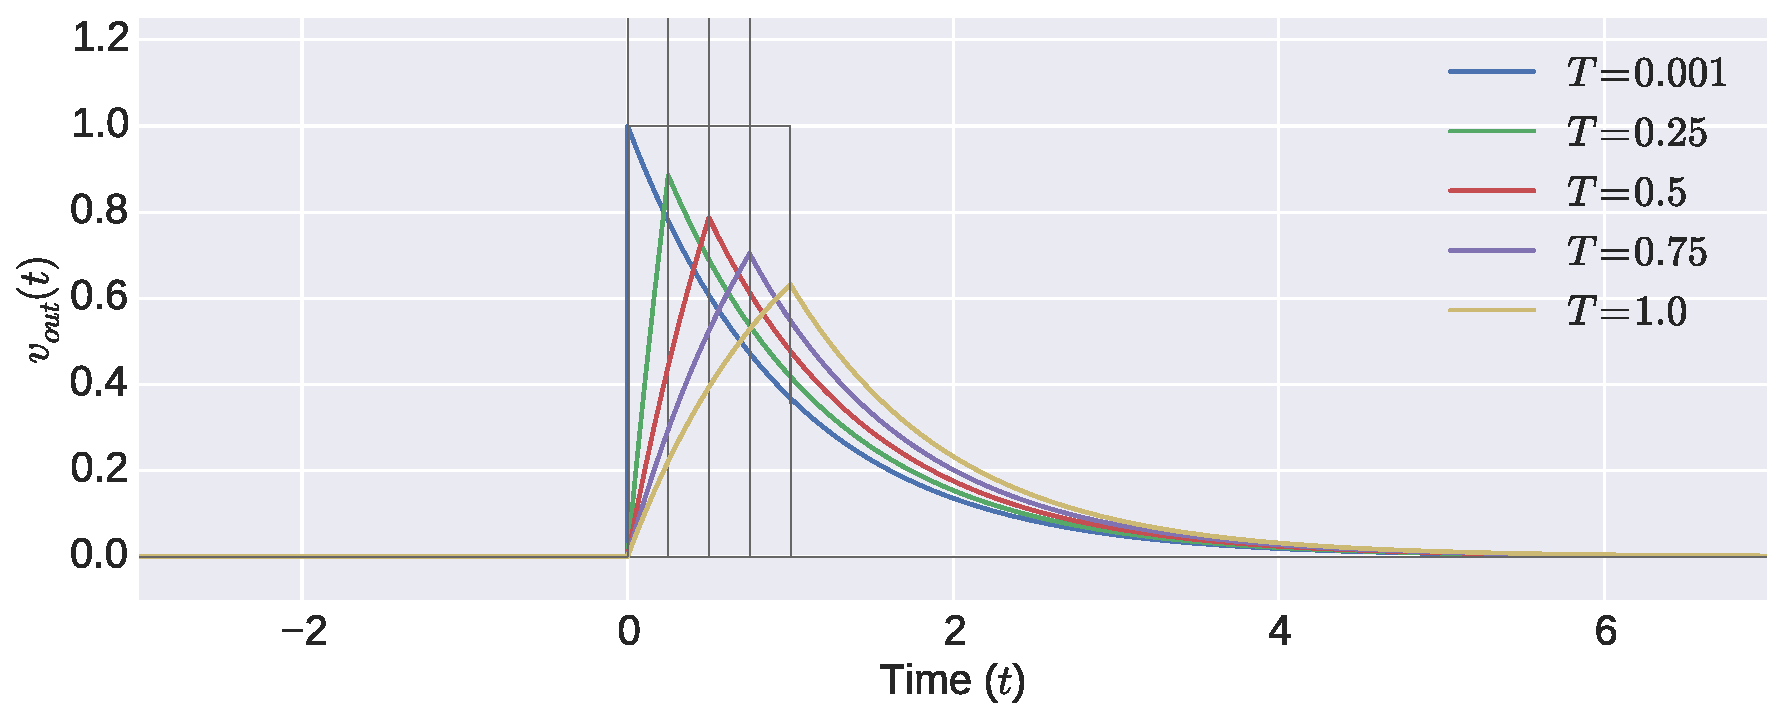
\includegraphics[width=\textwidth]{img/simple_rc.eps}
\end{figure}
\end{frame}

% IMPULSE RESPONSE AND SYSTEM PROPERTIES
\begin{frame}{Mechanics of the convolution integral}

Consider the signals,
\[ x(t) = \begin{cases}
1 & 0 \geq t \geq T1 \\
0 & \text{Otherwise}
\end{cases} \,\,\,\,\, y(t) = \begin{cases}
1 & 0 \geq t \geq T2 \\
0 & \text{Otherwise}
\end{cases} \]

How does the convolution integral do? 
\[ x(t) * y(t) = \int_{-\infty}^{\infty}x(\tau)y(t - \tau)d\tau \]
\pause
$x(t)*y(t)$ is the integral of the function $x(\tau)y(t - \tau)$.
\vspace{2mm}

\textbf{Note:} The integration is with respect to $\tau$, and $t$ is a constant as far as the integral is concerned.
\vspace{3mm}

\textbf{What is $x(t) * y(t)$?}
\end{frame}

% IMPULSE RESPONSE AND SYSTEM PROPERTIES
\begin{frame}{Impulse response act like a weighting function}

\begin{figure}
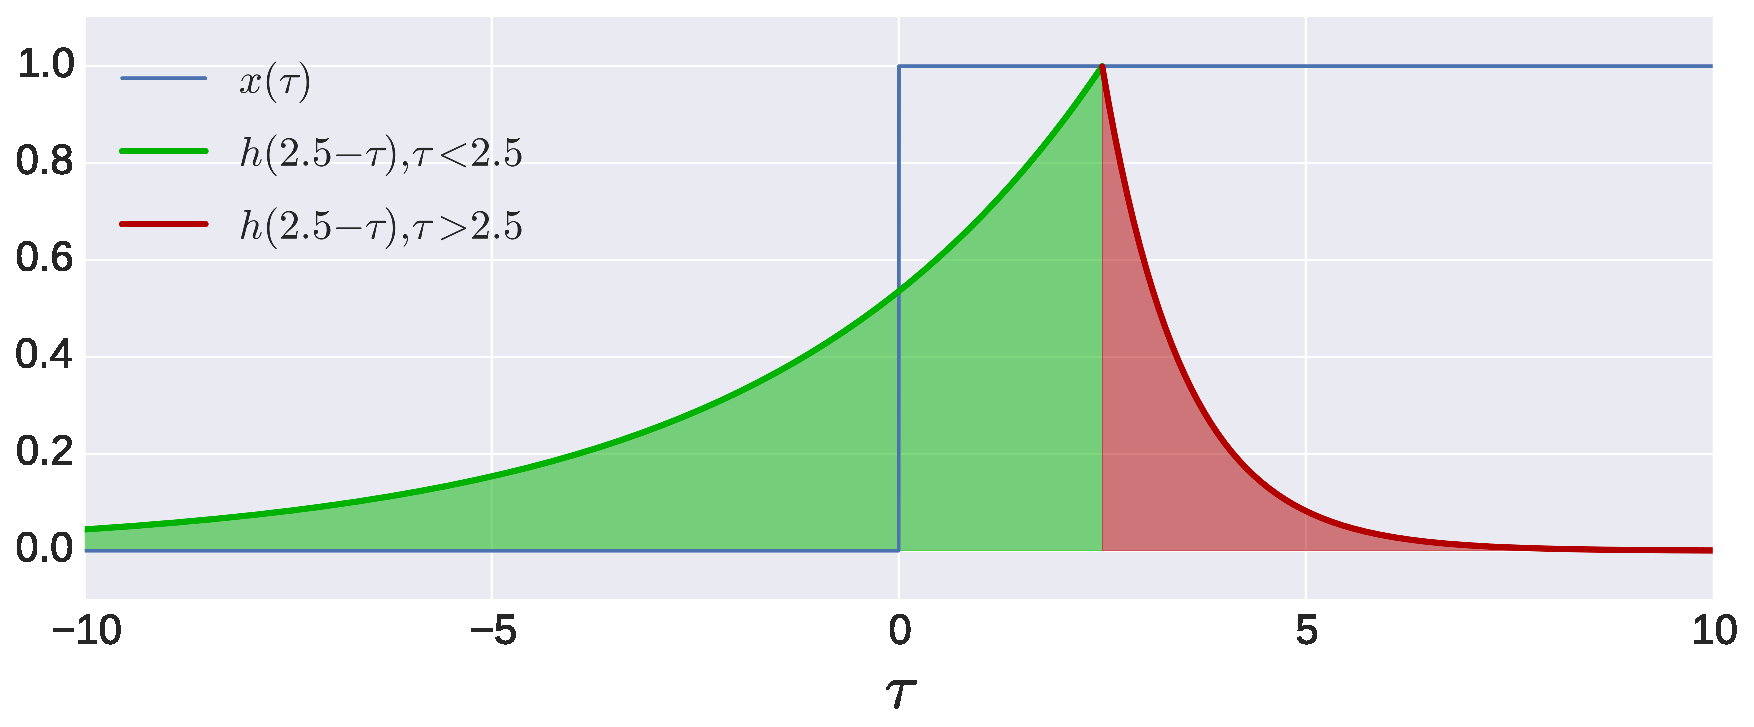
\includegraphics[width=\textwidth]{img/imp_resp_mech.eps}
\end{figure}

Here, $h(t) = \begin{cases}
e^{-t} & t < 0 \\
e^{-0.25t} & t \geq 0 \\
\end{cases}$ and $x(t) = u(t)$.

\vspace{2mm}

\[ \begin{cases}
h(t), \forall t < 0 & \text{Weightage for the future} \\
h(0) & \text{Weightage for the present} \\
h(t), \forall t > 0 & \text{Weightage for the past} \\
\end{cases} \]
\end{frame}

% IMPULSE RESPONSE AND SYSTEM PROPERTIES
\begin{frame}{Impulse response and LTI system properties}

\begin{itemize}
\item \textbf{(BIBO) Stability:} Let $\left|x(t)\right| < M_x, \,\,\, \forall t$, then $H$ is BIBO stable, iff $\left|y(t)\right| < \infty$, i.e.
\[ \int_{-\infty}^{\infty}\left|h(t)\right|dt < \infty \]
The \textbf{impulse response must be absolutely integrable}.

\item \textbf{Causality:} $h(t) = 0, \,\,\, \forall t < 0$.

\item \textbf{Memoryless:} $h(t) = k\delta(t)$.
\end{itemize}
\end{frame}

% DIFFERENTIAL EQUATIONS
\begin{frame}{Differential Equations}

Continuous-time LTI systems are often described by linear constant differential equations,

\[ \sum_{i=0}^{N-1}a_i\frac{d^i}{dt^i}y(t) = \sum_{j=0}^{M-1}b_j\frac{d^j}{dt^j}x(t) \]

The solution to this equation would provide the output for any given input, provided the appropriate initial conditions are available.

\[ y(t) = y_p(t) + y_h(t) \]

where, $y_p(t)$ is the particular solution, and $y_h(t)$ is the homogenous solution.
\end{frame}

% STATE SPACE REPRSENTATION
\begin{frame}{State space representation of LTI systems}
 
State space representation is a powerful and very useful tool in modern control theory.
\vspace{2mm}

Converts a $N^{th}$ order differential equation into $N$ $1^{st}$ order coupled differential equations.

\[ \sum_{i=0}^{N-1}a_i\frac{d^i}{dt^i}y(t) = \sum_{j=0}^{M-1}b_j\frac{d^j}{dt^j}x(t) \longrightarrow \begin{cases}
 \dot{\mathbf{x}}(t) = \mathbf{A}\mathbf{x}(t) + \mathbf{B}\mathbf{u}(t)\\
 \mathbf{y}(t) = \mathbf{C}\mathbf{x}(t) + \mathbf{D}\mathbf{u}(t)\\
\end{cases} \]

Here, $\mathbf{x}(t)$ is called the \textit{state} of the system, and $\mathbf{u}(t)$ is the \textit{input}, and $\mathbf{y}(t)$ is the \textit{output} of the system.

\end{frame}

% STATE SPACE REPRSENTATION
\begin{frame}{State space representation of LTI systems}
 
Why care about this representation?
\begin{itemize}
\item Gives insight into the internal behavior of the system.
\item Allows one to take the initial conditions of a system into account.
\item Allows handling of ``single input single output'' (SISO) and ``multi-input and multi-output'' (MIMO) under a single framework.
\end{itemize}

\textbf{Note:} The state of the system $\mathbf{x}(t)$ is not unique, and there are infinitely many choices.

\[ \tilde{\mathbf{x}}(t) = \mathbf{T}\mathbf{x}(t) \implies \begin{cases}
\dot{\tilde{\mathbf{x}}}(t) = \mathbf{T}\mathbf{A}\mathbf{T}^{-1}\tilde{\mathbf{x}}(t) + \mathbf{T}\mathbf{B}\mathbf{u}(t) \\
\mathbf{y}(t) = \mathbf{C}\mathbf{T}^{-1}\tilde{\mathbf{x}}(t) + \mathbf{D}\mathbf{u}(t) \\
\end{cases} \]
where, $\mathbf{T}$ is invertible.
\end{frame}

% STATE SPACE REPRSENTATION
\begin{frame}{State space representation of LTI systems}

What is the state-space representation of the following?
\[ \frac{d}{dt}y(t) + ay(t) = kx(t) \]

\[ a_2\frac{d^2}{dt^2}y(t) + a_1\frac{d}{dt}y(t) + a_2y(t) = bx(t) \]
\end{frame}

% BLOCK DIAGRAM REPRESENTATION
\begin{frame}{Block diagram Representation of LTI systems}

Given a pictorial representation of the internal structure of a given system.
\vspace{2mm}

Basic blocks required for block diagram representation:
\begin{itemize}
\item \textbf{Addition:} $ y(t) = \sum_{i} x_i(t) $
\item \textbf{Scalar multiplication:} $ y(t) = cx(t) $
\item \textbf{Integration:} $ y(t) = \int_{-\infty}^{t} x(\tau)d\tau $
\end{itemize}

This requires us to convert the differential equation to an integral equation.
\vspace{2mm}

\[ F(t) = \int_{-\infty}^{t} f(\tau)d\tau, \,\,\, f(t) = \frac{d}{dt}F(t) \]

What is the block diagram representation of the following system?
\[\frac{d}{dt}y\left(t\right) + ky\left(t\right) = x\left(t\right) \]

\end{frame}

\end{document}